%%%%%%%%%%%%%%%%%%%%%%%%%%%%%%%%%%%%%%%%%%%%%%%%%%%%%%%%%%%%%%%%%%%%%%
% LaTeX Example: Project Report
%
% Source: http://www.howtotex.com
%
% Feel free to distribute this example, but please keep the referral
% to howtotex.com
% Date: March 2011
%
%%%%%%%%%%%%%%%%%%%%%%%%%%%%%%%%%%%%%%%%%%%%%%%%%%%%%%%%%%%%%%%%%%%%%%
% How to use writeLaTeX:
%
% You edit the source code here on the left, and the preview on the
% right shows you the result within a few seconds.
%
% Bookmark this page and share the URL with your co-authors. They can
% edit at the same time!
%
% You can upload figures, bibliographies, custom classes and
% styles using the files menu.
%
% If you're new to LaTeX, the wikibook is a great place to start:
% http://en.wikibooks.org/wiki/LaTeX
%
%%%%%%%%%%%%%%%%%%%%%%%%%%%%%%%%%%%%%%%%%%%%%%%%%%%%%%%%%%%%%%%%%%%%%%
% Edit the title below to update the display in My Documents
%\title{Project Report}
%
%%% Preamble
\documentclass[paper=a4, fontsize=11pt]{scrartcl}
\usepackage[T1]{fontenc}
\usepackage{fourier}
\usepackage{float}

\usepackage[english]{babel}															% English language/hyphenation
\usepackage[protrusion=true,expansion=true]{microtype}
\usepackage{amsmath,amsfonts,amsthm} % Math packages
\usepackage[pdftex]{graphicx}
\usepackage{url}
%%%%%%%%%%%%%%%%%%%%%%%%%%%%%%%%%%%%%%%%%
% Lachaise Assignment
% Structure Specification File
% Version 1.0 (26/6/2018)
%
% This template originates from:
% http://www.LaTeXTemplates.com
%
% Authors:
% Marion Lachaise & François Févotte
% Vel (vel@LaTeXTemplates.com)
%
% License:
% CC BY-NC-SA 3.0 (http://creativecommons.org/licenses/by-nc-sa/3.0/)
% 
%%%%%%%%%%%%%%%%%%%%%%%%%%%%%%%%%%%%%%%%%

%----------------------------------------------------------------------------------------
%	PACKAGES AND OTHER DOCUMENT CONFIGURATIONS
%----------------------------------------------------------------------------------------

\usepackage{amsmath,amsfonts,stmaryrd,amssymb} % Math packages

\usepackage{enumerate} % Custom item numbers for enumerations

\usepackage[ruled]{algorithm2e} % Algorithms

\usepackage[framemethod=tikz]{mdframed} % Allows defining custom boxed/framed environments

\usepackage{listings} % File listings, with syntax highlighting
\lstset{
	basicstyle=\ttfamily, % Typeset listings in monospace font
}

%----------------------------------------------------------------------------------------
%	DOCUMENT MARGINS
%----------------------------------------------------------------------------------------

\usepackage{geometry} % Required for adjusting page dimensions and margins

\geometry{
	paper=a4paper, % Paper size, change to letterpaper for US letter size
	top=2.5cm, % Top margin
	bottom=3cm, % Bottom margin
	left=2.5cm, % Left margin
	right=2.5cm, % Right margin
	headheight=14pt, % Header height
	footskip=1.5cm, % Space from the bottom margin to the baseline of the footer
	headsep=1.2cm, % Space from the top margin to the baseline of the header
	%showframe, % Uncomment to show how the type block is set on the page
}

%----------------------------------------------------------------------------------------
%	FONTS
%----------------------------------------------------------------------------------------

\usepackage[utf8]{inputenc} % Required for inputting international characters
\usepackage[T1]{fontenc} % Output font encoding for international characters

\usepackage{XCharter} % Use the XCharter fonts

%----------------------------------------------------------------------------------------
%	COMMAND LINE ENVIRONMENT
%----------------------------------------------------------------------------------------

% Usage:
% \begin{commandline}
%	\begin{verbatim}
%		$ ls
%		
%		Applications	Desktop	...
%	\end{verbatim}
% \end{commandline}

\mdfdefinestyle{commandline}{
	leftmargin=10pt,
	rightmargin=10pt,
	innerleftmargin=15pt,
	middlelinecolor=black!50!white,
	middlelinewidth=2pt,
	frametitlerule=false,
	backgroundcolor=black!5!white,
	frametitle={Command Line},
	frametitlefont={\normalfont\sffamily\color{white}\hspace{-1em}},
	frametitlebackgroundcolor=black!50!white,
	nobreak,
}

% Define a custom environment for command-line snapshots
\newenvironment{commandline}{
	\medskip
	\begin{mdframed}[style=commandline]
}{
	\end{mdframed}
	\medskip
}

%----------------------------------------------------------------------------------------
%	FILE CONTENTS ENVIRONMENT
%----------------------------------------------------------------------------------------

% Usage:
% \begin{file}[optional filename, defaults to "File"]
%	File contents, for example, with a listings environment
% \end{file}

\mdfdefinestyle{file}{
	innertopmargin=1.6\baselineskip,
	innerbottommargin=0.8\baselineskip,
	topline=false, bottomline=false,
	leftline=false, rightline=false,
	leftmargin=2cm,
	rightmargin=2cm,
	singleextra={%
		\draw[fill=black!10!white](P)++(0,-1.2em)rectangle(P-|O);
		\node[anchor=north west]
		at(P-|O){\ttfamily\mdfilename};
		%
		\def\l{3em}
		\draw(O-|P)++(-\l,0)--++(\l,\l)--(P)--(P-|O)--(O)--cycle;
		\draw(O-|P)++(-\l,0)--++(0,\l)--++(\l,0);
	},
	nobreak,
}

% Define a custom environment for file contents
\newenvironment{file}[1][File]{ % Set the default filename to "File"
	\medskip
	\newcommand{\mdfilename}{#1}
	\begin{mdframed}[style=file]
}{
	\end{mdframed}
	\medskip
}

%----------------------------------------------------------------------------------------
%	NUMBERED QUESTIONS ENVIRONMENT
%----------------------------------------------------------------------------------------

% Usage:
% \begin{question}[optional title]
%	Question contents
% \end{question}

\mdfdefinestyle{question}{
	innertopmargin=1.2\baselineskip,
	innerbottommargin=0.8\baselineskip,
	roundcorner=5pt,
	nobreak,
	singleextra={%
		\draw(P-|O)node[xshift=1em,anchor=west,fill=white,draw,rounded corners=5pt]{%
		Question \theQuestion\questionTitle};
	},
}

\newcounter{Question} % Stores the current question number that gets iterated with each new question

% Define a custom environment for numbered questions
\newenvironment{question}[1][\unskip]{
	\bigskip
	\stepcounter{Question}
	\newcommand{\questionTitle}{~#1}
	\begin{mdframed}[style=question]
}{
	\end{mdframed}
	\medskip
}

%----------------------------------------------------------------------------------------
%	WARNING TEXT ENVIRONMENT
%----------------------------------------------------------------------------------------

% Usage:
% \begin{warn}[optional title, defaults to "Warning:"]
%	Contents
% \end{warn}

\mdfdefinestyle{warning}{
	topline=false, bottomline=false,
	leftline=false, rightline=false,
	nobreak,
	singleextra={%
		\draw(P-|O)++(-0.5em,0)node(tmp1){};
		\draw(P-|O)++(0.5em,0)node(tmp2){};
		\fill[black,rotate around={45:(P-|O)}](tmp1)rectangle(tmp2);
		\node at(P-|O){\color{white}\scriptsize\bf !};
		\draw[very thick](P-|O)++(0,-1em)--(O);%--(O-|P);
	}
}

% Define a custom environment for warning text
\newenvironment{warn}[1][Warning:]{ % Set the default warning to "Warning:"
	\medskip
	\begin{mdframed}[style=warning]
		\noindent{\textbf{#1}}
}{
	\end{mdframed}
}

%----------------------------------------------------------------------------------------
%	INFORMATION ENVIRONMENT
%----------------------------------------------------------------------------------------

% Usage:
% \begin{info}[optional title, defaults to "Info:"]
% 	contents
% 	\end{info}

\mdfdefinestyle{info}{%
	topline=false, bottomline=false,
	leftline=false, rightline=false,
	nobreak,
	singleextra={%
		\fill[black](P-|O)circle[radius=0.4em];
		\node at(P-|O){\color{white}\scriptsize\bf i};
		\draw[very thick](P-|O)++(0,-0.8em)--(O);%--(O-|P);
	}
}

% Define a custom environment for information
\newenvironment{info}[1][Info:]{ % Set the default title to "Info:"
	\medskip
	\begin{mdframed}[style=info]
		\noindent{\textbf{#1}}
}{
	\end{mdframed}
}
 % Include the file specifying the document structure and custom commands
\usepackage[ruled]{algorithm2e}


%%% Custom sectioning
\usepackage{sectsty}
\allsectionsfont{ \normalfont\scshape}


%%% Custom headers/footers (fancyhdr package)
\usepackage{fancyhdr}
\pagestyle{fancyplain}
\fancyhead{}											% No page header
\fancyfoot[L]{}											% Empty
\fancyfoot[C]{}											% Empty
\fancyfoot[R]{\thepage}									% Pagenumbering
\renewcommand{\headrulewidth}{0pt}			% Remove header underlines
\renewcommand{\footrulewidth}{0pt}				% Remove footer underlines
\setlength{\headheight}{13.6pt}


%%% Equation and float numbering
\numberwithin{equation}{section}		% Equationnumbering: section.eq#
\numberwithin{figure}{section}			% Figurenumbering: section.fig#
\numberwithin{table}{section}				% Tablenumbering: section.tab#


%%% Maketitle metadata
\newcommand{\horrule}[1]{\rule{\linewidth}{#1}} 	% Horizontal rule

\title{
		%\vspace{-1in}
		\usefont{OT1}{bch}{b}{n}
		\normalfont \normalsize \textsc{Stanford University} \\ [25pt]
		\horrule{0.5pt} \\[0.4cm]
		\huge CS221 Final Project - Impact Lens \\
		\horrule{2pt} \\[0.5cm]
}
\author{
		\normalfont 								\normalsize
        Nimisha Tandon\\[-3pt]		\normalsize
        Naman Muley\\[-3pt]		\normalsize
        Shaila Balaraddi\\[-3pt]		\normalsize
        \today
}
\date{}


%%% Begin document
\begin{document}
\maketitle
\section{Introduction}
A lot of information on the internet like news, social media posts etc that can impact brands. Directly, in the form of positive or negative PR and indirectly in that their product strategy could be potentially informed from these. Identifying such news is extremely useful for large brands or analytics divisions to get ahead of the PR cycle and formulate an early response.

\par We attempt to identify information that can be potentially impactful to a brand. We decided to tackle this problem by using classification algorithms and impact analysis methods. This project focuses on using classification to break down the documents into various categories and then look through the lens of a specific brand to calculate an impact score of each document. We present a stack rank of such documents back to the brand.

\section{Method Overview}
\paragraph{Approach}
This project can be broken down into two stages:
a) Classification : This is the component which given a bunch of documents is able to classify the category that they belongs to and give them a label.
b) Impact analysis. : This is the component, where given  an article/articles and a bunch of  words for the domain of the article, it is able to give an impact score for it , indicating how significant this article could be.

Both of these operations will deploy ML techniques. The system will take as input some domain data which represents the brand. It will also present to the user certain categories or news groups that the brand is interested in.

\begin{figure}
	\centering
 	 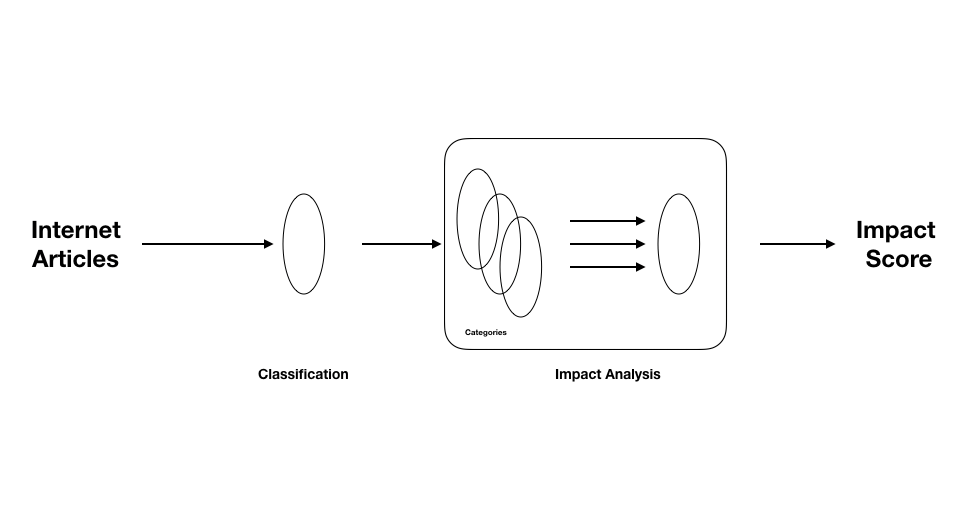
\includegraphics[width=0.6\linewidth]{impact_score.png}
	  \caption{Process Overview}
 	 \label{fig:Impact Potential}
\end{figure}
\section{Classification}
\subsubsection {Stochastic Gradient Descent with TFIDF Vectorizer}
{For classification of the documents into categories, we used the Logistic Regression classifier with TfIdf vectorizer which uses Stochastic Gradient Descent for optimization. SGD is a simple and efficient optimization method which is used for learning of linear classifiers.}

An SGD randomly chooses training data, gradually decreases the learning rate, and penalizes data points which deviate significantly from what's predicted. Since we had a large dataset to go through, SGD was the optimal and simplest algorithm to use.

For the purpose of this project we used the SGDClassifier provided by scikit-learn for training our models.

\subsubsection{Feature Extraction process}
TF-IDF which stands for Term Frequency – Inverse Document Frequency. It is one of the most important techniques used for information retrieval to represent how important a specific word or phrase is to a given document.

The tf-idf value increases in proportion to the number of times a word appears in the document but is often offset by the frequency of the word in the corpus, which helps to adjust with respect to the fact that some words appear more frequently in general.
\[tf(t,d) =  = \frac{\textit{no of occurrences of term in doc} }{\textit{total number of all words in document}}\]

\par Inverse document frequency

 This gives us the uniqueness of a word:

 \[idf(t,d) =  = log(\frac{\textit{no of times the term appears} }{\textit{no of documents containing the word}})\]
  \[TfIdf(t,d) =  = tf(t,d) * idf(t,d)\]

\subsubsection{Model fitting}
We then fit the model with pre-processed training data and labels. We feed the model with training data and their categories to train it to accurately classify the documents into respective categories.
\paragraph{Classify} We then run classification of test data on this trained model to get dataset categorized into various topics.

\textbf{Model Tuning and Optimization}
For the purpose of tuning the models , we used the Grid Search where the Hyper-parameters for training the models were varied and the best Hyper-parameters where chosen to finally build the model/s based on the outcome of the F1 score from Grid Search.  The table below talks about some of these hyper-parameters which were applied during building of the model and the impact of those parameters on the final F1 score.
\begin{figure}
	\centering
 	 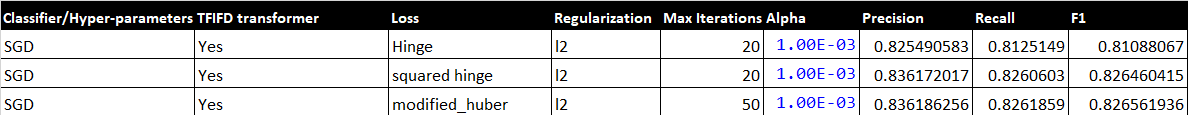
\includegraphics[width=0.9\linewidth]{Grid-Search.png}
	  \caption{Grid Search Results}
 	 \label{fig:Grid Search.png}
\end{figure}


\section{Impact score analysis}
\subsubsection {Similar Words using GloVe embeddings}
A measure of how relevant an article is to a brand is to know how many of semantically or linguistically similar words occur in that article. For each of the words in the vocabulary, we get a list of \textit{similar words} using the GloVe learning algorithm [1]. We then use a simple TF algorithm to understand how commonly do these similar words occur in an article.
\begin{center}
\begin{algorithm}
  \caption{Extend Vocabulary with Similar Words using Glove Model}
  \SetKwInOut{Input}{inputs}
  \SetKwInOut{Output}{output}
  \SetKwProg{GetGloveWords}{GetGloveWords}{}{}

 $Vocabulary \gets ["guns", "rifle", "weapon", "nra", "handgun", "firearm"] $\;
 $model \gets train\_glove(\textit{glove.6B.300d.w2vformat.tx}) $\;
 \GetGloveWords{$(Vocabulary, model)$} {
      $extended\_vocab \gets Vocabulary $\;
     \ForEach{word $w \in Vocabulary$}{%
       $similar\_words \gets model.get\_similar\_words($word=w, $topN=10) $\;
       $extended\_vocab.extend($similar\_words$) $\;
      }
    \KwRet{$extended\_vocab$}\;
  }
\end{algorithm}
\end{center}
Once the vocabulary is extended, we use this extended vocabulary to identify articles that have the most occurrences of these words. In the baseline program, we had used a similar algorithm to calculate, with the vocabulary as the raw input set of words. Following is a figure that shows how the expanded vocabulary behaves for a brand like NRA and input vocabulary = \textit {["guns", "weapons", "nra"]}.

\begin{figure}[ht]
	\centering
 	 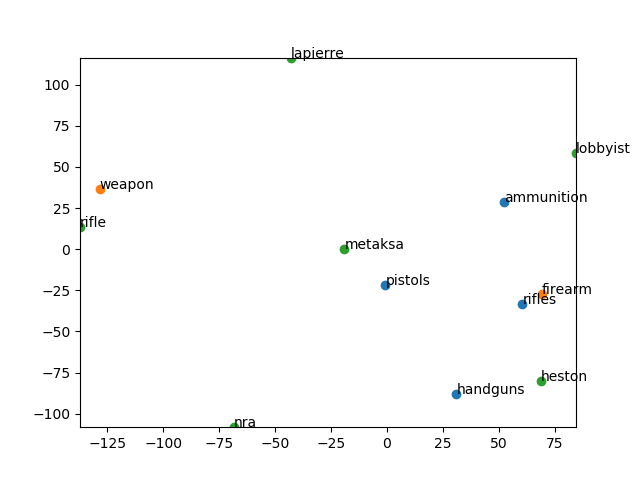
\includegraphics[width=0.5\linewidth]{similar_words_nra.png}
	  \caption{Similar Words obtained from GloVe Learning for \textit{NRA}}
 	 \label{fig:Similar Words for NRA}
\end{figure}

We use this extended vocabulary to come up with an impact score by simply counting frequencies of these words. Our algorithm that performs this to come up with an impact score for each article in the category is given below. The score dictionary contains the impact score calculated for each article in the set of articles.

\begin {center}
\begin {algorithm}[ht]
\SetNoFillComment
\caption{Calculate Impact Score for each article from a list of articles, given extended vocabulary}
\SetKwInOut{Input}{inputs}
\SetKwInOut{Output}{output}
\SetKwProg{CalculateVocabImpactScore}{CalculateVocabImpactScore}{}{}
\CalculateVocabImpactScore{$(V, D)$} {
    \Input{A list of words that form ExtendedVocabulary V; a list of articles D}
    \Output{A dictionary representing impact scores for all articles in D}
    $score \gets \emptyset $\;
    $RangeD \gets range(0, len(D)) $\;
    \ForEach {index $i \in RangeD$} {
    	score[i] = 0 \;
	freq = [] \;
	\tcc{iterate over all words in $i_{th}$ article to count frequency}
	\ForEach {word $w \in D[i]$} {
		freq[word] += 1 \;
	}
	\tcc{iterate over all words in V to build a score for article $i$}
	\ForEach {word $w \in V$} {
		score[i] += freq[w] \;
	}
    }
    score.Normalize() \;
    \KwRet{$score$}\;
}
\end {algorithm}
\end {center}

We have detailed our results of the above score dictionary in the Results section.

\subsubsection {Relevant words using TF}

Term Frequency is used to find the frequency of vocabulary words in a document to perform impact score analysis by extracting relevancy from a document.
Before using TF to calculate, we perform a basic text pre processing on the categorized documents.
\begin{itemize}
\item {Remove all stop words.(ex: in, the, are it)}
\item {Convert all words to lowercase.}
\end {itemize}
We then use the term frequency calculation to calculate the impact score..
\begin{itemize}
\item {Term Frequency}
\[tf(t,d) =  = \frac{\textit{no of occurrences of term in doc} }{\textit{total number of all words in document}}\]
\end{itemize}



\section{Data}
We used the following data sets for various learning algorithms.

\begin {enumerate}

\item \textbf{\textit{20-News:} }
The newsgroup data set contains 18000 news posts on 20 topics split. We used this data set to train the classifier and to come up with fundamental categories for the news articles.

The categories provided by this data set seemed to work just fine for our purposes. Following are the categories that this data set provides. To showcase our system and it's functionalities, we created a fictitious client NRA and chose the \textit{talk.politics.guns} category to work upon in detail.

\begin {enumerate}
\item {comp.graphics}
\item {comp.os.ms-windows.misc}
\item {comp.sys.ibm.pc.hardware}
\item {comp.sys.mac.hardware}
\item {comp.windows.x}
\item {misc.forsale}
\item {rec.autos}
\item {rec.motorcycles}
\item {rec.sport.baseball}
\item {rec.sport.hockey}
\item {talk.politics.misc}
\item {talk.politics.guns}
\item { talk.politics.mideast}
\item {sci.crypt}
\item {sci.electronics}
\item {sci.med}
\item {sci.space}
\item {talk.religion}
\item {alt.atheism}
\item {soc.religion.christian}
\end {enumerate}

We used the 20 News group to also assess accuracy of our classifiers. The test data split out of this dataset was used to assess the accuracy of the classifiers.

\item \textbf{\textit{Wikipedia 2014 + Gigaword 5}}
The GloVe enhancement used the Wikipedia 2014 dataset with 300 dimensional vectors. This dataset helps get a set of enhanced positive words that complement a given word. For the input set of words, we find the positive GloVe embeddings and include them in an enhanced vocabulary, which we can then use for impact score algorithms.

\item \textbf{\textit{New York Times articles:}}
A set of 6179 articles from New York Times archive of December 2018. These provide a perfect testing dataset to see how our system classifies articles into categories and provides impact scores for each.

\end {enumerate}

\section{Experiments}
Below are some of things we tried in addition to those listed above, however did not chose to include them in the main flow because of lack of good results using the same.
1. Aspect extraction and their polarity extraction for Impact Analysis.
\begin{figure}[H]
	\centering
 	 
\includegraphics[width=0.6\linewidth]{Aspect_Extraction.png}
	  \caption{Aspect and Polarity of Aspect Extraction}
 	 \label{fig:Aspect Extraction.png}
\end{figure}
Aspect is
For the purpose of extracting the impact score it seemed almost natural to think of some things about the product and or brand in question that the people would be talking about. Which led us to the notion of extracting Aspects from the articles and then studying its polarity in order to further understand if that aspect is being positively or negatively perceived.

As described in the diagram above, Aspects were extracted using a very rudimentary approach:
{Step 1: Here we clean the articles, by removing all stop words}
{Step 2: We then tokenize the articles using a Sentence tokenizer}
{Step 3: POS Tagging for each token in the sentence were then identified.}
{Step 4: We then filtered those tokens which were Noun and Noun Phrases}
{Step 5: Using the tokens which were nouns or noun phrases we then identify the Aspects and also the associated orientation/polarity.}

{After passing the articles through the pipeline of the aspect and sentiment extraction, below are some of the results that were obtained:}

\begin{figure}[H]
	\centering
 	 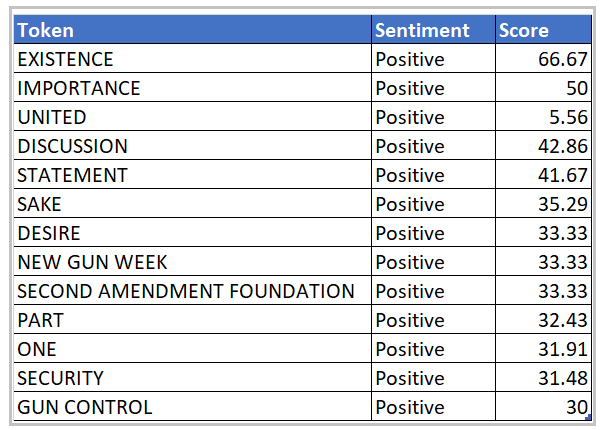
\includegraphics[width=0.6\linewidth]{Aspect_Scores.png}
	  \caption{Aspects and Polarity Score of Aspects}
 	 \label{fig:Aspect Extraction.png}
\end{figure}

As the results indicate, since the aspect extraction is purely based on the Noun words and Noun phrases, they are not all truly aspects.
Additionally some of these identified as Aspects do not depict the correct polarity hence we decided to not include these results in the main stream for calculating the impact score.

\section{Results}
We wanted to showcase a few sets of results from our experiments.


\subsection {Classification: Naive Bayes vs. Stochastic Gradient Descent}
The SGD classifier did slightly better than the Naive Bayes classifier. We used the test data split in the News20 group dataset to test out our classification and verify with the labels already present in the dataset.

\par The Naive Bayes classifier had an accuracy of 0.80 and the SGD classifier with hinge loss had an accuracy of 0.82. We believe that is too close a difference to conclusively say one is better than another.

\subsection {New York Times results}

The NYT archive of 2018 December provided a great real world ground for our complete end-to-end testing. We went with the fictitious scenario that NRA is our client and they have selected the category \textit{guns}. They have then provided the following set of words as vocabulary: \textit{["guns", "shooting", "lobby", "rifles", "weapon", "nra", "handgun", "politics"]}

Following were some of the noteworthy results:

\begin{figure}[H]
	\centering
 	 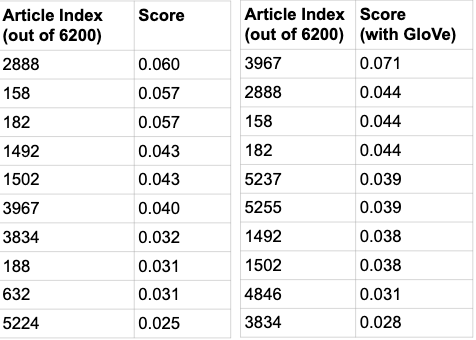
\includegraphics[width=0.6\linewidth]{nyt_articles_stackrank.png}
	  \caption{NYT Articles Stack Rank Without GloVe embeddings and With Glove Embeddings}
 	 \label{fig:NYT Articles}
\end{figure}

\begin {itemize}
\item {\textbf{\textit{Classification}}} The SGD classified 189 articles into the \textit{talk.politics.guns} category. Articles were on variety of topcis like gun shootings, poaching in africa, drug cartels around the world, police aggression in US etc. All of these were rightly classified.

\item {\textbf{\textit{Impact Scores}}}
\par We found the impact scores change after enhancing the vocabulary with GloVe embeddings. With the raw input vocabulary, the articles that came in the top 10 index included the following:

\begin {enumerate}
\item Article 2888: Mass shootings in Parkland, FL and gun restrictions
\item Article 158: Police shootings of black population
\item Article 3967: Nigerian Military shooting unarmed protesters
\end {enumerate}

\par After the use of GloVe embeddings, with the vocabulary that included the positive GloVe embeddings, we found the articles change impact scores. New articles came into the top 10, while those that were present changed their positions. For example we now found \textit{Article 3957 - Use of American guns in poaching in Mozambique} entering into the top 10. This article talks about shipment of American guns being sent over for illegal activities in Africa and can be important from a strategy perspective for NRA, our fictitious client.

\end{itemize}

\section{Conclusion}
\section{References}


%%% End document
\end{document}